% ------------------------------------------------------------------------
% ------------------------------------------------------------------------
% abnTeX2: Modelo de Trabalho Academico (tese de doutorado, dissertacao de
% mestrado e trabalhos monograficos em geral) em conformidade com
% ABNT NBR 14724:2011: Informacao e documentacao - Trabalhos academicos -
% Apresentacao
% ------------------------------------------------------------------------
% ------------------------------------------------------------------------

\documentclass[
	% -- opções da classe memoir --
	12pt,				% tamanho da fonte
	openright,			% capítulos começam em pág ímpar (insere página vazia caso preciso)
	twoside,			% para impressão em recto e verso. Oposto a oneside
	a4paper,			% tamanho do papel.
	% -- opções da classe abntex2 --
	%chapter=TITLE,		% títulos de capítulos convertidos em letras maiúsculas
	%section=TITLE,		% títulos de seções convertidos em letras maiúsculas
	%subsection=TITLE,	% títulos de subseções convertidos em letras maiúsculas
	%subsubsection=TITLE,% títulos de subsubseções convertidos em letras maiúsculas
	% -- opções do pacote babel --
	english,			% idioma adicional para hifenização
	brazil,				% o último idioma é o principal do documento
	svgnames
	]{abntex2}\usepackage[]{graphicx}\usepackage[]{color}
% maxwidth is the original width if it is less than linewidth
% otherwise use linewidth (to make sure the graphics do not exceed the margin)
\makeatletter
\def\maxwidth{ %
  \ifdim\Gin@nat@width>\linewidth
    \linewidth
  \else
    \Gin@nat@width
  \fi
}
\makeatother

\definecolor{fgcolor}{rgb}{0.345, 0.345, 0.345}
\newcommand{\hlnum}[1]{\textcolor[rgb]{0.686,0.059,0.569}{#1}}%
\newcommand{\hlstr}[1]{\textcolor[rgb]{0.192,0.494,0.8}{#1}}%
\newcommand{\hlcom}[1]{\textcolor[rgb]{0.678,0.584,0.686}{\textit{#1}}}%
\newcommand{\hlopt}[1]{\textcolor[rgb]{0,0,0}{#1}}%
\newcommand{\hlstd}[1]{\textcolor[rgb]{0.345,0.345,0.345}{#1}}%
\newcommand{\hlkwa}[1]{\textcolor[rgb]{0.161,0.373,0.58}{\textbf{#1}}}%
\newcommand{\hlkwb}[1]{\textcolor[rgb]{0.69,0.353,0.396}{#1}}%
\newcommand{\hlkwc}[1]{\textcolor[rgb]{0.333,0.667,0.333}{#1}}%
\newcommand{\hlkwd}[1]{\textcolor[rgb]{0.737,0.353,0.396}{\textbf{#1}}}%
\let\hlipl\hlkwb

\usepackage{framed}
\makeatletter
\newenvironment{kframe}{%
 \def\at@end@of@kframe{}%
 \ifinner\ifhmode%
  \def\at@end@of@kframe{\end{minipage}}%
  \begin{minipage}{\columnwidth}%
 \fi\fi%
 \def\FrameCommand##1{\hskip\@totalleftmargin \hskip-\fboxsep
 \colorbox{shadecolor}{##1}\hskip-\fboxsep
     % There is no \\@totalrightmargin, so:
     \hskip-\linewidth \hskip-\@totalleftmargin \hskip\columnwidth}%
 \MakeFramed {\advance\hsize-\width
   \@totalleftmargin\z@ \linewidth\hsize
   \@setminipage}}%
 {\par\unskip\endMakeFramed%
 \at@end@of@kframe}
\makeatother

\definecolor{shadecolor}{rgb}{.97, .97, .97}
\definecolor{messagecolor}{rgb}{0, 0, 0}
\definecolor{warningcolor}{rgb}{1, 0, 1}
\definecolor{errorcolor}{rgb}{1, 0, 0}
\newenvironment{knitrout}{}{} % an empty environment to be redefined in TeX

\usepackage{alltt}

% ---
% Novo list of (listings) para QUADROS
% ---

%\newcommand{\quadroname}{Quadro}
%\newcommand{\listofquadrosname}{Lista de quadros}

%\newfloat[chapter]{quadro}{loq}{\quadroname}
%\newlistof{listofquadros}{loq}{\listofquadrosname}
%\newlistentry{quadro}{loq}{0}

% configurações para atender às regras da ABNT
%\counterwithout{quadro}{chapter}
%\renewcommand{\cftquadroname}{\quadroname\space}
%\renewcommand*{\cftquadroaftersnum}{\hfill--\hfill}

% ---
% PACOTES
% ---

% ---
% Pacotes fundamentais
% ---
\usepackage{lmodern}			% Usa a fonte Latin Modern
\usepackage[T1]{fontenc}		% Selecao de codigos de fonte.
\usepackage[utf8]{inputenc}		% Codificacao do documento (conversão automática dos acentos)
\usepackage{indentfirst}		% Indenta o primeiro parágrafo de cada seção.
\usepackage{color}			% Controle das cores
\usepackage{graphicx}			% Inclusão de gráficos
\usepackage{microtype} 			% para melhorias de justificação
\usepackage{setspace}
\usepackage{wrapfig}

% ---
% Para titulo em destaque sem sequencia de numeração
% ---
\newcommand{\datatitle}[1]{
  \normalsize \textsc{#1}
}

% ---
% Funções matematicas
% ---
\usepackage{amsmath,amssymb,amstext}
\usepackage{mathtools}                  % Funcionalidades (como \dcases)
\usepackage{dsfont}    %% Para \mathds{1} Indicadora
\usepackage{bm}

\DeclareMathOperator{\Ell}{\mathcal{L}}
\DeclareMathOperator{\R}{\mathbb{R}}
\DeclareMathOperator{\ind}{\mathds{1}}

\DeclareRobustCommand{\rchi}{{\mathpalette\irchi\relax}}
\newcommand{\irchi}[2]{\raisebox{\depth}{$#1\chi$}}

% ---
% Para tabelas
% ---
\usepackage{multirow}
\usepackage{array}
\usepackage{threeparttable}

% ---
% Pacotes e definições adcionais, para adequações especificas
% ---
\usepackage{tikz}
\usepackage{pdflscape}			% para ambiente landscape
\usepackage{pgfgantt}			% cronograma estilo gráfico de gantt
\usepackage{multicol}
\usetikzlibrary{backgrounds}
\usepackage{tasks}

% ---
% Fontes matemáticas
% ---
\usepackage{mathpazo}
\usepackage{inconsolata}
\usepackage{verbatim}

% ---
% Pacotes adicionais, usados apenas no âmbito do Modelo Canônico do abnteX2
% ---
\usepackage{lipsum}				% para geração de dummy text
% ---

% ---
% Pacotes de citações
% ---
\usepackage[brazilian,hyperpageref]{backref}% Paginas com as citações
\usepackage[alf, abnt-etal-list=0]{abntex2cite}				% Citações padrão ABNT

% ---
% CONFIGURAÇÕES DE PACOTES
% ---

% ---
% Configurações do pacote backref
% Usado sem a opção hyperpageref de backref
\renewcommand{\backrefpagesname}{Citado na(s) página(s):~}
% Texto padrão antes do número das páginas
\renewcommand{\backref}{}
% Define os textos da citação
\renewcommand*{\backrefalt}[4]{
  \ifcase #1 %
  Nenhuma citação no texto.%
  \or
  Citado na página #2.%
  \else
  Citado #1 vezes nas páginas #2.%
  \fi}%
% ---

% ---
% Informações de dados para CAPA e FOLHA DE ROSTO
% ---
\titulo{Aprendizado de máquina \\ Laboratório 1 - Impactos da Representação}
\vspace{2cm}
\autor{Lineu Alberto Cavazani de Freitas}
\local{Curitiba}
\data{2021}
\instituicao{Universidade Federal do Paraná}

\preambulo{Relatório apresentado à disciplina
    Aprendizado de Máquina do Programa de Pós Graduação em Informática da Universidade Federal do Paraná.}
% ---

% ---
% Configurações de aparência do PDF final

% informações do PDF
\makeatletter
\hypersetup{
  % pagebackref=true,
  pdftitle={\@title},
  pdfauthor={\@author},
  pdfsubject={\imprimirpreambulo},
  pdfcreator={LaTeX with abnTeX2},
  % pdfkeywords={abnt}{latex}{abntex}{abntex2}{projeto de pesquisa},
  colorlinks=true,	% false: boxed links; true: colored links
  linkcolor=blue,     % color of internal links
  citecolor=blue, % color of links to bibliography
  filecolor=magenta, % color of file links
  urlcolor=black,
  bookmarksdepth=4
}
\addto\captionsbrazil{
  \renewcommand{\bibname}{REFER\^ENCIAS}
}
\makeatother
% ---

% ---
% Espaçamentos entre linhas e parágrafos
% ---

% O tamanho do parágrafo é dado por:
\setlength{\parindent}{1.3cm}

% Controle do espaçamento entre um parágrafo e outro:
\setlength{\parskip}{0.2cm}  % tente também \onelineskip

% ---
% Highlight knitr code (pode-usar usar os varios highligths já definidos
% com thm = knit_theme$get("nuvola"); knit_theme$set(thm))
% ---

\renewcommand{\hlnum}[1]{\textcolor[rgb]{0.733,0,1}{#1}}%
\renewcommand{\hlstr}[1]{\textcolor[rgb]{0,0.533,0}{#1}}%
\renewcommand{\hlcom}[1]{\textcolor[rgb]{0,0,0}{#1}}%
\renewcommand{\hlopt}[1]{\textcolor[rgb]{0.412,0.412,0.412}{#1}}%
\renewcommand{\hlstd}[1]{\textcolor[rgb]{0.2,0.2,0.2}{{#1}}}%
\renewcommand{\hlkwa}[1]{\textcolor[rgb]{0.2,0.2,0.2}{{#1}}}%
\renewcommand{\hlkwb}[1]{\textcolor[rgb]{0.4,0,0}{\textbf{#1}}}%
\renewcommand{\hlkwc}[1]{\textcolor[rgb]{0.13,0.29,0.53}{#1}}%
\renewcommand{\hlkwd}[1]{\textcolor[rgb]{0.13,0.29,0.53}{\textbf{#1}}}%

% ---
% compila o indice
% ---
\makeindex
% ---

% ----
% Início do documento
% ----
\IfFileExists{upquote.sty}{\usepackage{upquote}}{}
\begin{document}

% Seleciona o idioma do documento (conforme pacotes do babel)
% \selectlanguage{english}
\selectlanguage{brazil}

% Retira espaço extra obsoleto entre as frases.
\frenchspacing

% ----------------------------------------------------------
% ELEMENTOS PRÉ-TEXTUAIS
% ----------------------------------------------------------
% \pretextual

% ---
% Capa
% ---
\tikz[remember picture,overlay] \node[opacity=1,inner sep=0pt] at
(current page.center){
  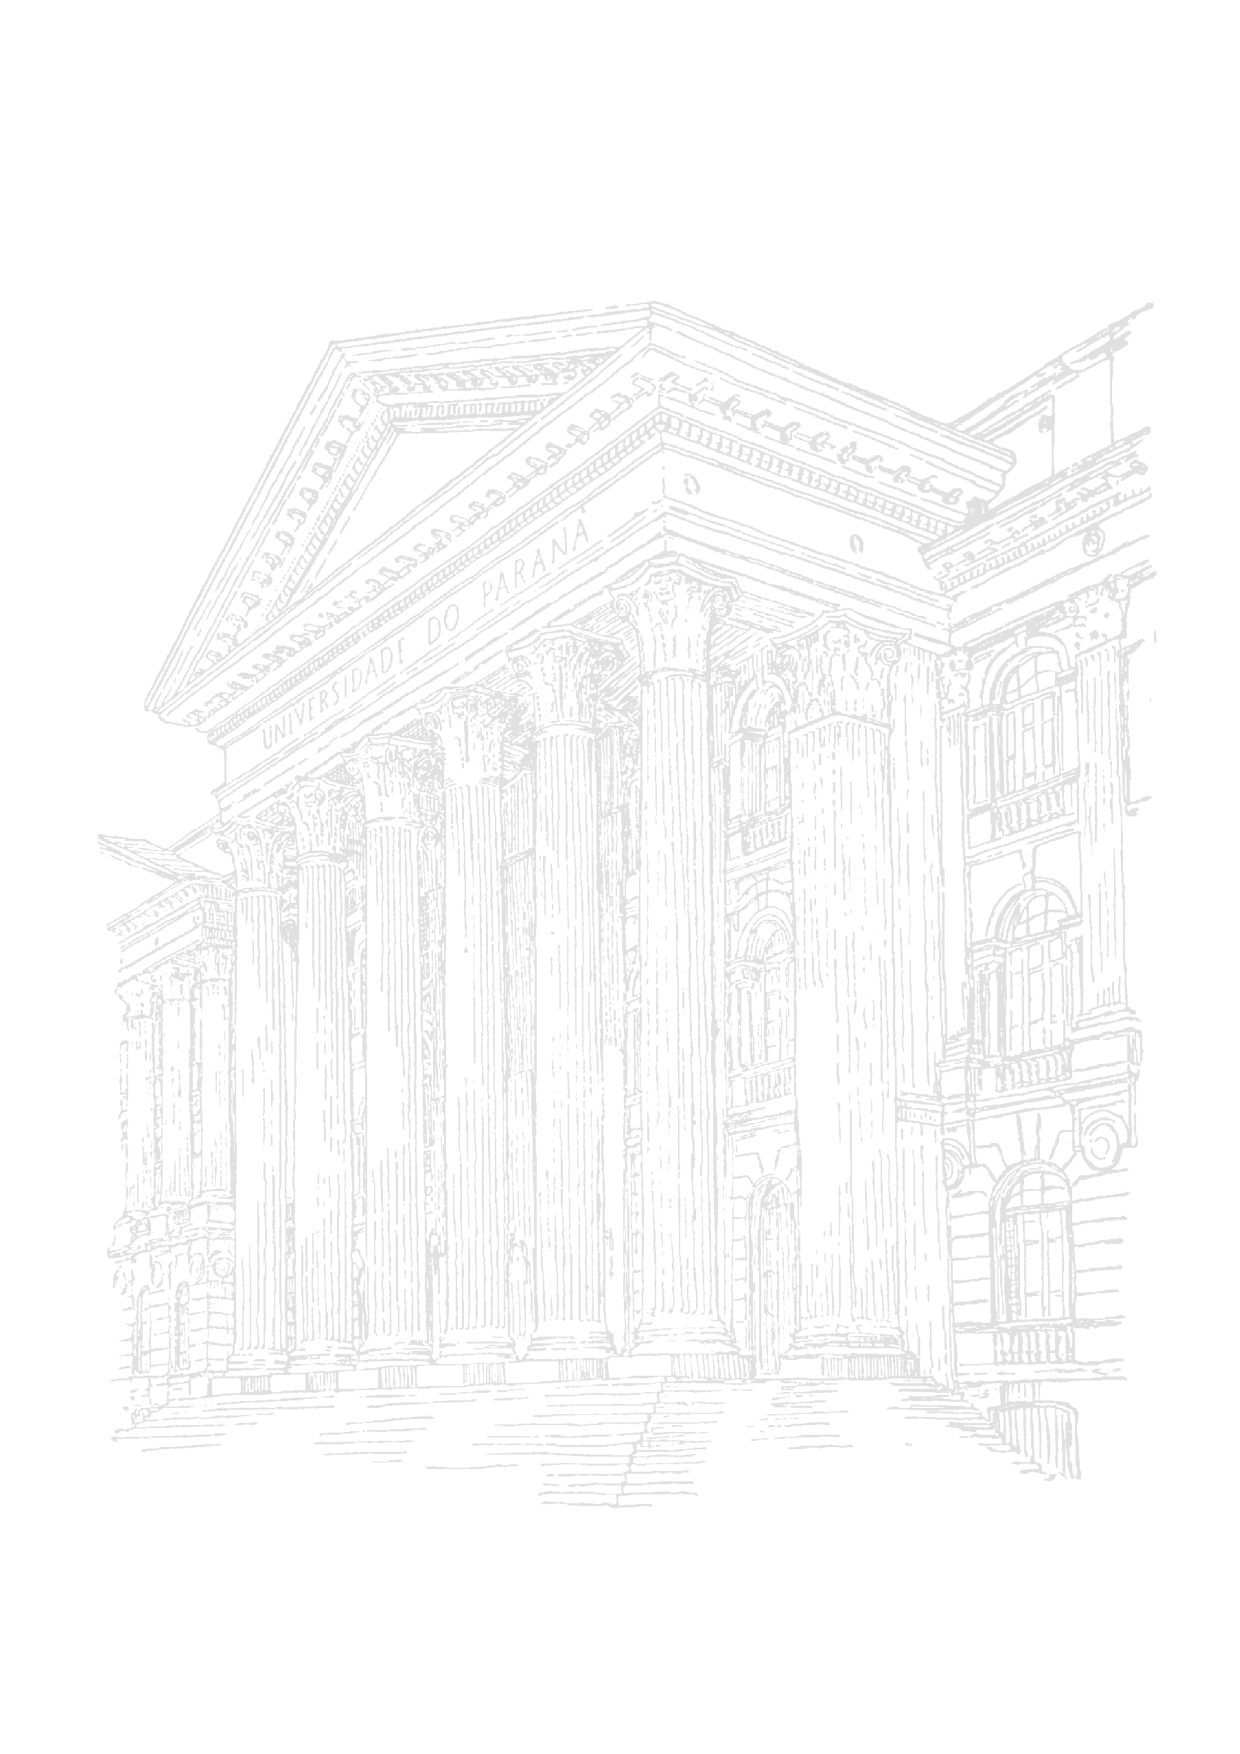
\includegraphics[width=\paperwidth,
  height=\paperheight]{images/ufpr_bg}};

\begin{center}
  {\Large \textsf{Universidade Federal do Paraná}}
  \vspace{-0.5cm}
\end{center}

\imprimircapa

% ---

% ---
% Folha de rosto
% ---
\imprimirfolhaderosto
% ---

% ---
% Dedicatória
% ---
% \begin{dedicatoria}
%   \lipsum[1]
% \end{dedicatoria}
% ---

% ---
% Agradecimentos
% ---
% \begin{agradecimentos}
%   \lipsum[1]
% \end{agradecimentos}
% ---

% ---
% Epígrafe
% ---
%\begin{epigrafe}
%    \vspace*{\fill}
%	\begin{flushright}
%          \textit{``Software is like sex: it's better when \\
%            it's free``}\\
%          --- Linus Torvalds \\[1cm]

%          \textit{``The numbers are where the scientific \\ discussion
%            should start, not end.''}\\
%          --- Steven N. Goodman
%	\end{flushright}
%\end{epigrafe}
% ---

% ---
% RESUMOS
% ---

% resumo em português
%\setlength{\absparsep}{18pt} % ajusta o espaçamento dos parágrafos do resumo
%\begin{resumo}


% ---
% inserir lista de ilustrações
% ---
%\pdfbookmark[0]{\listfigurename}{lof}
%\listoffigures*
%\cleardoublepage
% ---

% ---
% inserir lista de tabelas
% ---
%\pdfbookmark[0]{\listtablename}{lot}
%\listoftables*
%\cleardoublepage
% ---

% ---
% inserir lista de quadros
% ---
%\pdfbookmark[0]{\listofquadrosname}{loq}
%\listofquadros*
%\cleardoublepage
% ---

% ---
% inserir lista de abreviaturas e siglas
% ---
% \begin{siglas}
%   \item[ABNT] Associação Brasileira de Normas Técnicas
%   \item[abnTeX] ABsurdas Normas para TeX
% \end{siglas}
% ---

% ---
% inserir lista de símbolos
% ---
% \begin{simbolos}
%   \item[$ \log $] Logarítmo neperiano (de base $e$).
%   \item[$ \ell $] log-verossimilhança maximizada.
%   \item[AIC] Critério de Informação de Akaike, do inglês \textit{Akaike
%       Information Criterion}.
% \end{simbolos}
% ---

% ---
% inserir o sumario
% ---
\pdfbookmark[0]{\contentsname}{toc}
\tableofcontents*
\cleardoublepage
% ---

% ----------------------------------------------------------
% ELEMENTOS TEXTUAIS
% ----------------------------------------------------------
\textual

\chapter{Introdução}
\label{cap:introducao}

% ----------------------------------------------------------------------
% CAPÍTULO 1INTRODUÇÃO
% ----------------------------------------------------------------------

Aprendizado de máquina

Classificadores

KNN

Reconhecimento de dígitos manuscritos

Extração de características de imagens

Objetivo da atividade

\chapter{Descrição das atividades}
\label{cap:conjuntos-de-dados}

% ----------------------------------------------------------------------
% CAPÍTULO 2 - DESCRIÇÃO DAS ATIVIDADES
% ----------------------------------------------------------------------

Descrição da atividade

\chapter{Resultados obtidos}
\label{cap:revisao-de-literatura}

% ----------------------------------------------------------------------
% CAPÍTULO 3 - RESULTADOS OBTIDOS
% ----------------------------------------------------------------------

Resultados obtidos

\chapter{Discussão dos resultados }
\label{cap:estudo-de-simulacao}

% ------------------------------------------------------------------------
% CAPÍTULO 4 - DISCUSSÃO
% ------------------------------------------------------------------------

Discussão

\chapter{Considerações finais}
\label{cap:resultados-e-discussao}

% ----------------------------------------------------------------------
% CAPÍTULO 5 - CONCLUSÃO
% ----------------------------------------------------------------------

Conclusão

% ---
\phantompart

% ---
% Conclusão
% ---

% ----------------------------------------------------------
% ELEMENTOS PÓS-TEXTUAIS
% ----------------------------------------------------------
\postextual

% ----------------------------------------------------------
% Referências bibliográficas
% ----------------------------------------------------------

%% Utilize este na elaboração do documento
\bibliography{refs}

%% Utilize este apenas ao final, quando não forem mais realizadas
%% alterações
% \begin{flushleft}
%   \small
% \renewcommand\refname{}
% \vspace*{-1.5cm}
% \input{01-tcc_corrigido.bbl}
% \end{flushleft}

% ----------------------------------------------------------
% Apêndices
% ----------------------------------------------------------

% ---
% Inicia os apêndices
% ---
% \begin{apendicesenv}

% Imprime uma página indicando o início dos apêndices
% \partapendices

% \chapter{Programas R}
% \label{capA:codigostcc}

% \end{apendicesenv}
% ---

% ----------------------------------------------------------
% Anexos
% ----------------------------------------------------------

%% % ---
%% % Inicia os anexos
%% % ---
%% \begin{anexosenv}
%% % Imprime uma página indicando o início dos anexos
%% \partanexos
%% \chapter{Lipsum}
%% \lipsum[30]
%% \end{anexosenv}

%---------------------------------------------------------------------
% INDICE REMISSIVO
%---------------------------------------------------------------------
% \phantompart
% \printindex
%---------------------------------------------------------------------

\end{document}
